\documentclass[12pt,t]{beamer}

%------------------------------------------------------------------------------
% configuration
%------------------------------------------------------------------------------
\RequirePackage{etex}
\usepackage{../../themes/dbt}
\usepackage{catchfilebetweentags}

\setbeameroption{hide notes}

\graphicspath{{images/}}

% a few macros
\newcommand{\bi}{\begin{itemize}}
\newcommand{\ei}{\end{itemize}}
\newcommand{\ig}{\includegraphics}
\newcommand{\incnote}[1]{\note{\ExecuteMetaData[notes.tex]{#1}}}

%------------------------------------------------------------------------------
% title
%------------------------------------------------------------------------------
% slide
\title{Systèmes d'exploitation pour l'embarqué}
\subtitle{UV 5.2 - Exécution et Concurrence}

\author{\href{}{Paul Blottière}}
\institute{
    \href{http://www.ensta-bretagne.fr/}{ENSTA Bretagne} \\[2pt]
    \href{}{\tt \scriptsize 10 Novembre 2015}
}
\date{
    \href{https://github.com/pblottiere}{\tt \scriptsize https://github.com/pblottiere}
}

% info
\begin{document}

{
\setbeamertemplate{footline}{} % no page number here
\frame{
    \titlepage
    \incnote{title}
} }

%------------------------------------------------------------------------------
% amélioration continue
%------------------------------------------------------------------------------
\begin{frame}{Amélioration continue}
    \subt{Contributions}
    \vspace{12pt}

    \begin{center}
    
\includegraphics[scale=0.7]{github.png}
    \end{center}

    \bi
    \itemsep12pt
    \item Dépôt du cours : \href{https://github.com/pblottiere/embsys}{\tt \scriptsize https://github.com/pblottiere/embsys}
    \item Souhaits d'amélioration, erreurs, ... : ouverture d'issues (avec le bon tag!)
    \item Apports de correction : Pull Request
    \ei
\end{frame}

%------------------------------------------------------------------------------
% organisation
%------------------------------------------------------------------------------
\begin{frame}{Organisation}
    \vspace{12pt}

    \bi
        \itemsep12pt
        \item 9 CM
        \item 6 TE
        \item 2 BE
    \ei

    \incnote{organisation}
\end{frame}

%------------------------------------------------------------------------------
% plan
%------------------------------------------------------------------------------
\begin{frame}{Plan}
    \subt{}

    \bi
        \itemsep8pt
        \item Un peu d'histoire
        \item Les normes
        \item Logiciel Libre et Logiciel Open-Source
        \item Licences de distribution
        \item Définitions et propriétés
        \item Architectures matérielles
        \item Quelques chiffres
        \item Les OS embarqués existant
        \item Comment choisir?
        \item Et si on choisit Linux?
    \ei

    \note {
    }
\end{frame}

%------------------------------------------------------------------------------
% histoire1
%------------------------------------------------------------------------------
\begin{frame}{Un peu d'histoire}
    \subt{Le premier jeu vidéo}
    \vspace{20pt}

    \begin{columns}[onlytextwidth]
        \begin{column}{0.45\textwidth}
            \centering
            1964 : Multics \\
            \vspace{30pt}
            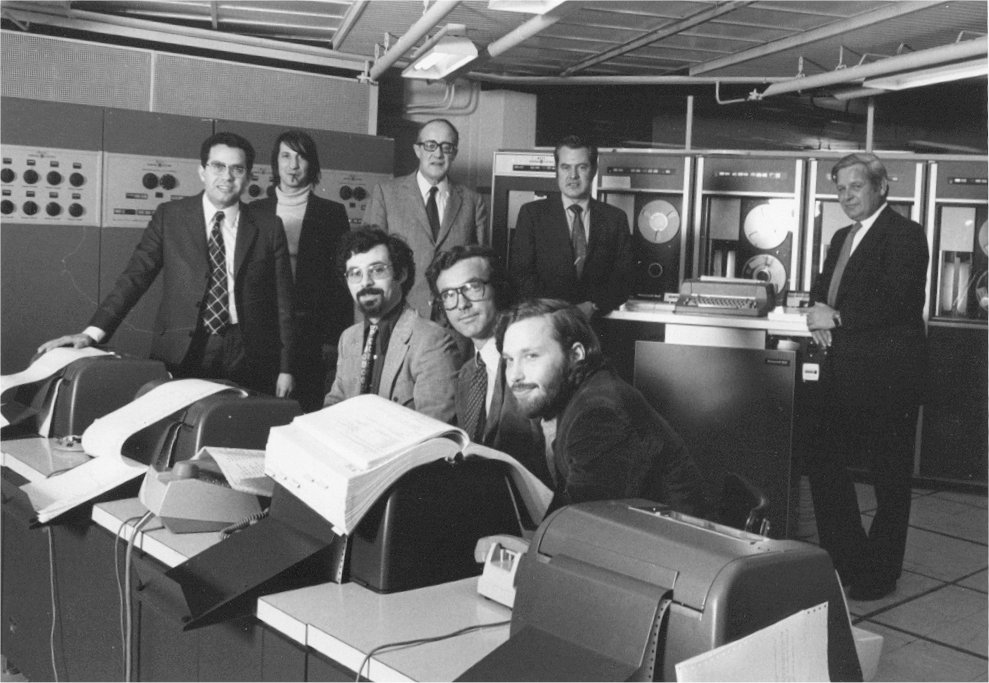
\includegraphics[scale=0.15]{ge645-paris.jpg}
        \end{column}
        \begin{column}{0.45\textwidth}
            \centering
            1969 : Space Travel par Ken Thompson \\
            \vspace{20pt}
            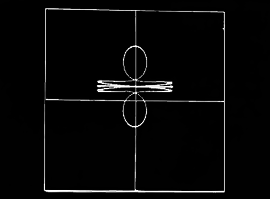
\includegraphics[scale=0.6]{space-travel.png}
        \end{column}
    \end{columns}

    \incnote{histoire1}
\end{frame}

%------------------------------------------------------------------------------
% histoire2
%------------------------------------------------------------------------------
\begin{frame}{Un peu d'histoire}
    \subt{La naissance du langage C}
    \vspace{30pt}

    \begin{columns}[onlytextwidth]
        \begin{column}{0.45\textwidth}
            \centering
            1971 : Le C par Dennis Ritchie \\
            \vspace{20pt}
            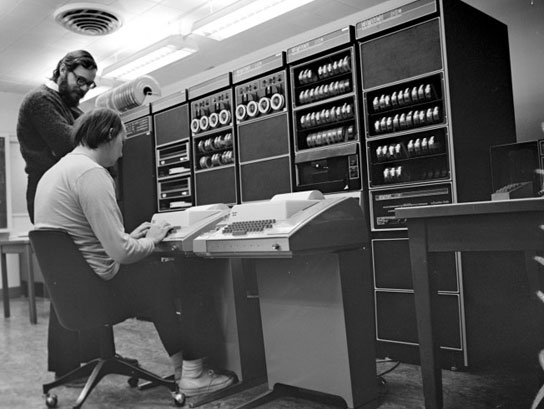
\includegraphics[scale=0.3]{ken-ritchie-1972.jpg}
        \end{column}
        \begin{column}{0.45\textwidth}
            \centering
            1983 : GNU par Stallman \\
            \vspace{20pt}
            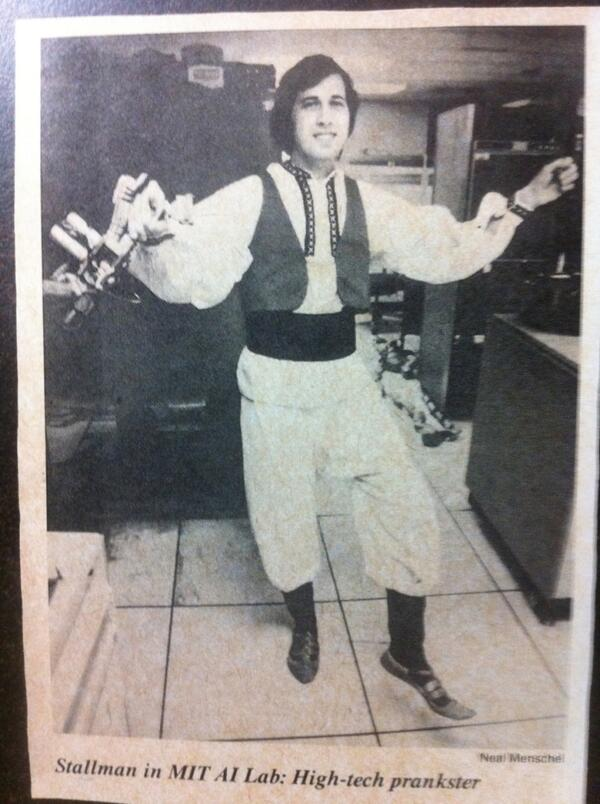
\includegraphics[scale=0.15]{rms-mitlab.jpg}
        \end{column}
    \end{columns}

    \incnote{histoire2}
\end{frame}

%------------------------------------------------------------------------------
% histoire3
%------------------------------------------------------------------------------
\begin{frame}{Un peu d'histoire}
    \subt{Un hobby devenu célèbre}
    \vspace{30pt}

    \begin{columns}[onlytextwidth]
        \begin{column}{0.45\textwidth}
            \centering
            1987 : Linux par Linus Torvalds \\
            \vspace{20pt}
            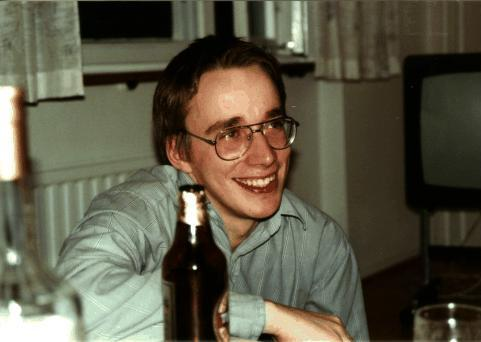
\includegraphics[scale=0.3]{linus.jpg}
        \end{column}
        \begin{column}{0.45\textwidth}
            \centering
            1992 : GNU / Linux \\
            \vspace{30pt}
            
\includegraphics[scale=0.2]{gnu-linux.png}
        \end{column}
    \end{columns}

    \incnote{histoire3}
\end{frame}

%------------------------------------------------------------------------------
% histoire4
%------------------------------------------------------------------------------
\begin{frame}{Un peu d'histoire}
    \subt{De nos jours}
    \vspace{5pt}

    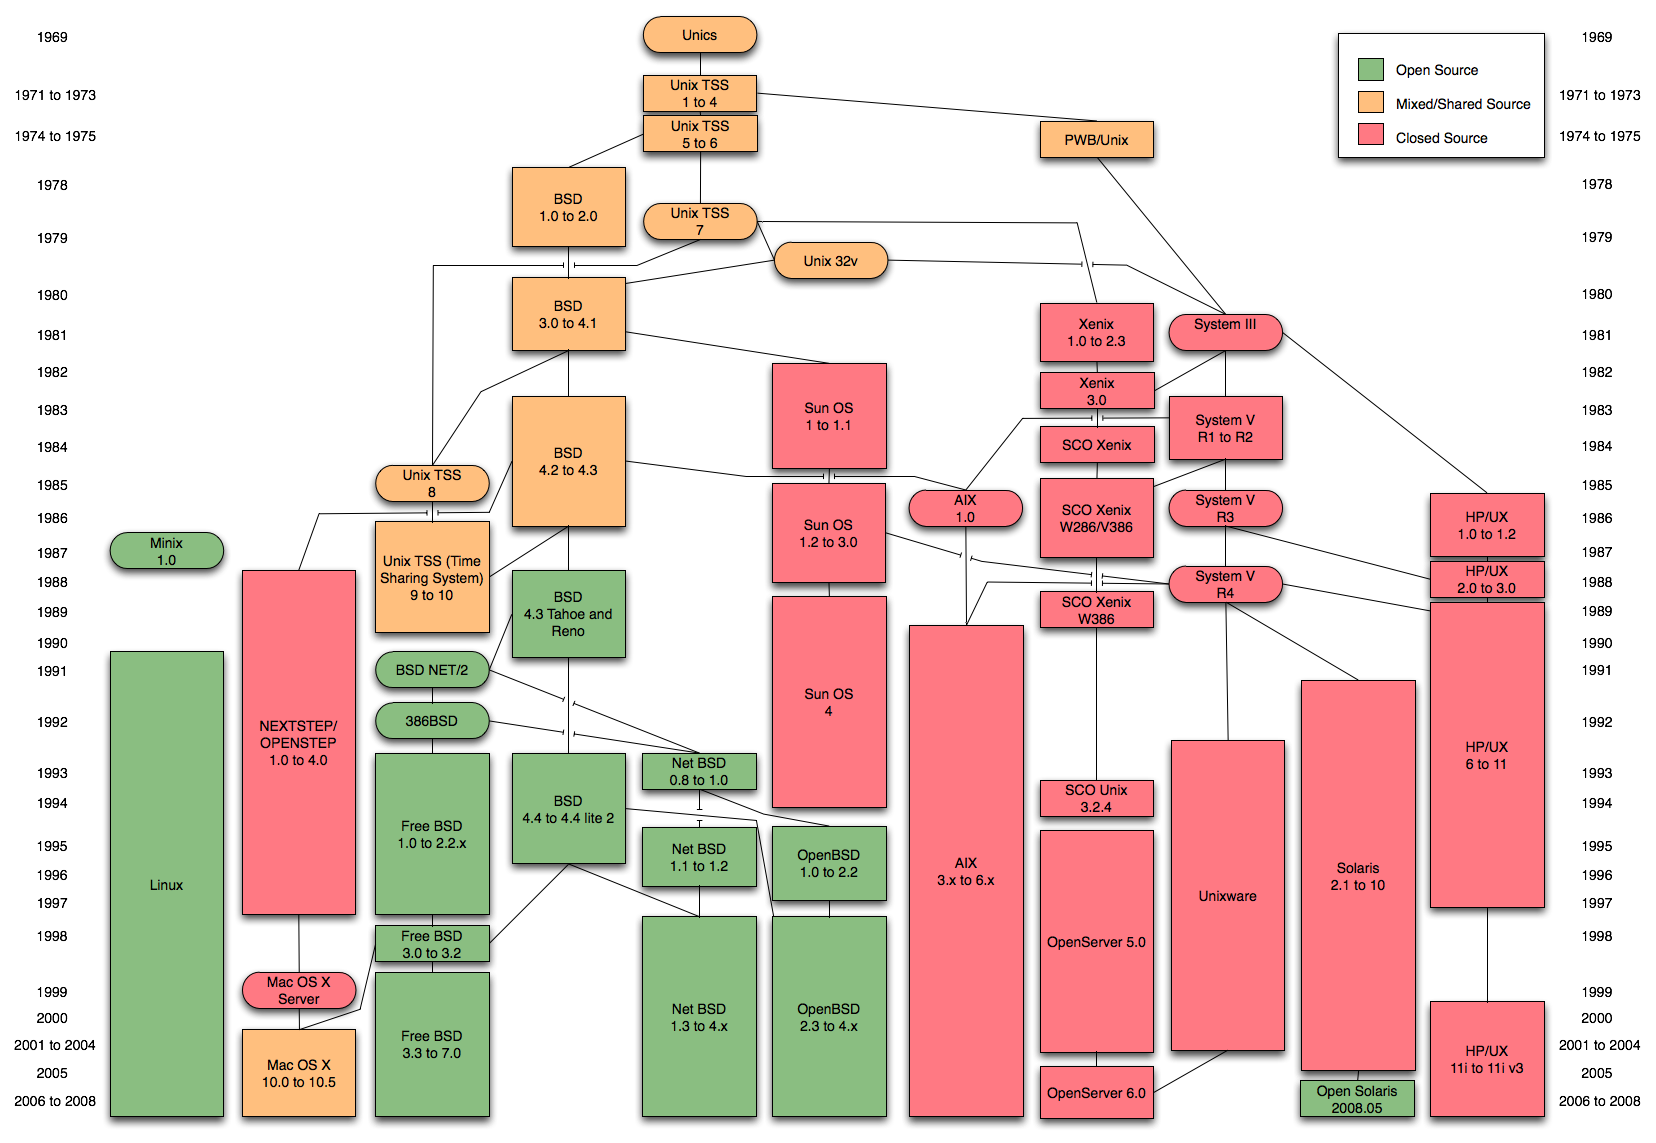
\includegraphics[scale=0.18]{timeline.png}

    \incnote{histoire4}
\end{frame}

%------------------------------------------------------------------------------
% normes1
%------------------------------------------------------------------------------
\begin{frame}{Les normes}
    \subt{SUSv3}
    \vspace{20pt}

    Des normes sont nécessaires pour assurer une compatibilité des logiciels
    entre systèmes d'exploitation:
    \vspace{10pt}
    \bi
    \itemsep12pt
    \item 1988 : Portable Operating System Interface (POSIX). Plusieurs versions : 1,
                 1.b, 1.c
      \item 1997 : UNIX98 ou Single UNIX Specification V2
    \item Standard actuel : SUS V3 (fusion entre POSIX et UNIX98)
    \ei

    \vspace{10pt}
    \centering
    \href{http://www.unix.org/version3/}{\tt \scriptsize http://www.unix.org/version3/}

    \incnote{normes1}
\end{frame}

%------------------------------------------------------------------------------
% normes2
%------------------------------------------------------------------------------
\begin{frame}[fragile]{Les normes}
    \subt{POSIXLY\_CORRECT SIR!}
    \vspace{10pt}

    POSIX:
    \begin{lstlisting}[language=bash]
    tool [-a][-b][-c option_argument] \
        [-d|-e][-f[option_argument]][operand...]
    \end{lstlisting}

    \vspace{10pt}
    Sous GNU/Linux, les règles sont différentes!

    \vspace{10pt}
    Conséquences sous GNU/Linux:

    \begin{lstlisting}
    # ls -a .
    .vimrc .vim devel doc
    # ls . -a
    .vimrc .vim devel doc
    # POSIXLY_CORRECT=1 ls . -a
    ls: impossible d'accéder à -a: Aucun fichier ou
        dossier de ce type
    .vimrc .vim devel doc
    \end{lstlisting}

    \incnote{normes2}
\end{frame}

%------------------------------------------------------------------------------
% opensource
%------------------------------------------------------------------------------
\begin{frame}{Logiciel Libre et Logiciel Open Source}
    \subt{Question de philosophie...}
    \incnote {opensource}
\end{frame}

%------------------------------------------------------------------------------
% licences1
%------------------------------------------------------------------------------
\begin{frame}{Licences de distribution}
    \subt{Copyleft, GPL, LGPL, ...}
    \incnote {licences1}
\end{frame}

%------------------------------------------------------------------------------
% licences2
%------------------------------------------------------------------------------
\begin{frame}{Licences de distribution}
    \subt{Conséquences dans la vie courante...}
    \incnote{licences2}
\end{frame}

%------------------------------------------------------------------------------
% def1
%------------------------------------------------------------------------------
\begin{frame}{Définitions et propriétés}
    \subt{Le Kernel et système d'exploitation}
    \incnote{def1}
\end{frame}

%------------------------------------------------------------------------------
% def2
%------------------------------------------------------------------------------
\begin{frame}{Définitions et propriétés}
    \subt{Dans le monde des systèmes embarqués...}
    \incnote{def2}
\end{frame}

%------------------------------------------------------------------------------
% def3
%------------------------------------------------------------------------------
\begin{frame}{Définitions et propriétés}
    \subt{Dans le monde des systèmes embarqués...}
    \incnote{def3}
\end{frame}

%------------------------------------------------------------------------------
% def4
%------------------------------------------------------------------------------
\begin{frame}{Définitions et propriétés}
    \subt{microcontrolleur vs microprocesseur}
    \incnote{def4}
\end{frame}

%------------------------------------------------------------------------------
% chiffres1
%------------------------------------------------------------------------------
\begin{frame}{Quelques chiffres}
    \subt{Les systèmes embarqués sont partout!}
    \incnote{chiffres1}
\end{frame}

%------------------------------------------------------------------------------
% chiffres2
%------------------------------------------------------------------------------
\begin{frame}{Quelques chiffres}
    \subt{Soutien des états}
    \incnote{chiffres2}
\end{frame}

%------------------------------------------------------------------------------
% chiffres3
%------------------------------------------------------------------------------
\begin{frame}{Quelques chiffres}
    \subt{Répartition du Chiffre d'Affaires}
    \incnote{chiffres3}
\end{frame}

%------------------------------------------------------------------------------
% chiffres4
%------------------------------------------------------------------------------
\begin{frame}{Quelques chiffres}
    \subt{Répartition des effectifs}
    \incnote{chiffres4}
\end{frame}

%------------------------------------------------------------------------------
% embos1
%------------------------------------------------------------------------------
\begin{frame}{Les OS embarqués existant}
    \subt{Sans base Linux}
    \incnote{embos1}
\end{frame}

%------------------------------------------------------------------------------
% embos2
%------------------------------------------------------------------------------
\begin{frame}{Les OS embarqués existant}
    \subt{A base de Linux}
    \incnote{embos2}
\end{frame}

%------------------------------------------------------------------------------
% choice1
%------------------------------------------------------------------------------
\begin{frame}{Comment choisir?!}
    \subt{Systèmes propriétaires ?}
    \incnote{choice1}
\end{frame}

%------------------------------------------------------------------------------
% choice2
%------------------------------------------------------------------------------
\begin{frame}{Comment choisir?}
    \subt{Systèmes Open Source?}
    \incnote{choice2}
\end{frame}

%------------------------------------------------------------------------------
% linux1
%------------------------------------------------------------------------------
\begin{frame}{Et si on choisit Linux...}
    \subt{Avantages}
    \incnote{linux1}
\end{frame}

%------------------------------------------------------------------------------
% linux2
%------------------------------------------------------------------------------
\begin{frame}{Et si on choisit Linux...}
    \subt{Avantages}
    \incnote{linux2}
\end{frame}

%------------------------------------------------------------------------------
% linux3
%------------------------------------------------------------------------------
\begin{frame}{Et si on choisit Linux...}
    \subt{Inconvénients}
    \incnote{linux3}
\end{frame}

%------------------------------------------------------------------------------
% hard1
%------------------------------------------------------------------------------
\begin{frame}{Aspect matériel}
    \subt{Processeurs}
    \incnote{hard1}
\end{frame}

%------------------------------------------------------------------------------
% hard2
%------------------------------------------------------------------------------
\begin{frame}{Aspect matériel}
    \subt{MMU}
    \incnote{hard2}
\end{frame}

\end{document}
